%%%%%%%%%%%%%%%%%%%%%%%%%%%%%%%%%%%%%%%%%%%
% Partie non numérotée, mais présente dans le sommaire
\setcounter{part}{-1}
\part{Module Presentation}
\begin{frame}{About me}
    \begin{itemize}
%    \item \structure{Study:} Univ. St-Étienne (1999), PhD (2003). HPC.
    \item \structure{Since Feb. 2005:} Associate Professor at Université de
      Lorraine)\\
      \structure{Teaching:} {\small Télécom Nancy}, \structure{Research:}
      {\small AlGorille team (LORIA = UL/INRIA/CNRS)}
    \end{itemize}
    
  \begin{columns}
    \begin{column}{.27\linewidth}
      \begin{tikzpicture}[xscale=1,yscale=1]
        \node (nodehost) [name=nodehost] 
          { 
\includegraphics[height=23mm]{img/laptop.png}};

        \node (nodelisting) [above right= -25mm of nodehost]%, overlay]  
          { 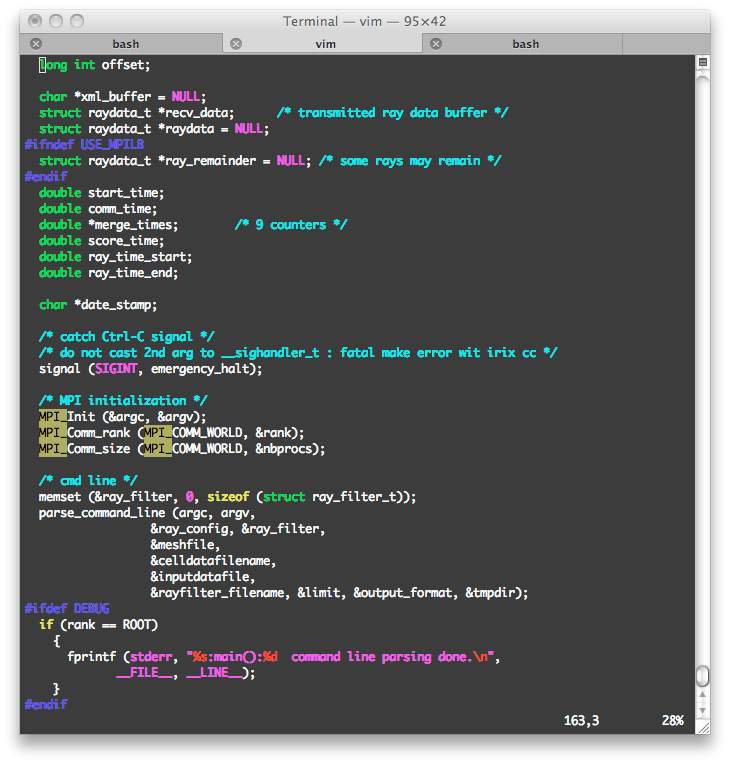
\includegraphics[height=12mm]{img/mpi-codelisting.png}};

        \node (nodeimagine) [
          shape             = cloud callout,
          cloud puffs       = 11,
          aspect            = 1.5,
          opacity           =.75,
          draw              = black!90!white, % colour of the border
          top color         = white,                % | filling of the node
          bottom color      = black!30!white, % |
          text              = black!90!white, % colour of the fonts
          thick,                              % thickness of the border
          above             = 5mm of nodehost,
          minimum height    = 25mm,
          minimum width     = 30mm,
          callout relative pointer={(285:5.5mm)},
        ]{};

        \node at (nodeimagine) {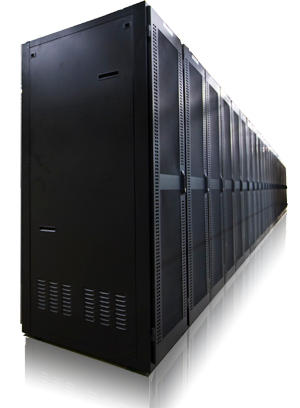
\includegraphics[width=15mm]{img/cluster.png}};
      \end{tikzpicture}
    \end{column}
    \begin{column}{.72\linewidth}
      \begin{block}{Research: {\color{black}Experimental methodologies}}
        \begin{itemize} 
        \item Assess distributed applications {\small(perfs, bugs)}
        \item SimGrid project: Simulator of distributed systems\\
          Correct modeling, efficient simulation
        \item Formal verification (model-checking)
        \end{itemize}
      \end{block}\vspace{-.5\baselineskip}

      \begin{block}{Teachings: {\color{black}Programming and Algorithms}}
        \begin{itemize}
        \item Introduction, Java/Scala, AlgoProg, C 2nd language
        \item System Prog; Ex-\{Algo dist, P2P, Distributed Prog\}
        \item PLM: Programmer's Learning Machine
        \end{itemize}
      \end{block}

      \structure{\large Outreach:} Unplugged Computer Science, etc.
    \end{column}
  \end{columns}
  \bigskip
  \begin{itemize}
    \item \structure{More info:}
      {\small\url{http://www.loria.fr/~quinson/} (\url{Martin.Quinson@loria.fr})}
    \end{itemize}
\end{frame}
%%%%%%%%%%%%%%%%%%%%%%%%%%%%%%%%%%%%%%%%%%%%%%%%%%%%%%%%%%%%%%%%%%%%%%%%%%%%%%%
\begin{frame}[squeeze]{About this module: \alert{Algorithmic and Programming}}
  \begin{block}{Programming? Let the computer do your work!}
    \begin{itemize}
    \item[] ~\vspace{-\baselineskip}
      \begin{itemize}
      \item How to explain what to do?
      \item How to make sure that it does what it is supposed to? That
        it is efficient?
      \item What if it does not?
      \end{itemize}
    \end{itemize}
  \end{block}
  \vspace{-.5\baselineskip}

  \begin{block}<2->{Module content and goals: }
    \begin{itemize}
    \item Introduction to Algorithmic
      \begin{itemize}
      \item Master theoretical basements (computer science is a science)
      \item Know some classical problem resolution techniques
      \item Know how to evaluate solutions (correctness, performance)
      \end{itemize}

    \item First steps in programming: learn-by-doing activity (you need to \textit{practice})
    \end{itemize}
  \end{block}
  \vspace{-.5\baselineskip}

  \begin{block}<3->{Other modules at Telecom Nancy}
    \begin{itemize}
    \item Prerequisites
      \begin{itemize}
      \item Tactical programming in Scala: \texttt{if}, \texttt{for}, methods
      \item Sense of logic, intuition (good math background helps)
      \end{itemize}
    \item Afterward: Object Oriented Programming; Object-Oriented Design

      \medskip
    \item[] {\small(please be patient, it's our second time with TOP before OOP)}
    \end{itemize}
  \end{block}
\end{frame}
%%%%%%%%%%%%%%%%%%%%%%%%%%%%%%%%%%%%%%%%%%%%%%%%%%%%%%%%%%%%%%%%%%%%%%%%%%
\begin{frame}{Module organization}
  \begin{block}{Time organization}
    \begin{itemize}
    \item 6 two-hours lectures {\small(CM, with Martin Quinson)}: 
      Concepts introduction
    \item 10 two-hours exercise session {\small(TD, with staff member%
      \footnote{ ~Olivier Festor, Sébastien Da Silva, Martin Quinson.}%
      )}: Theoretical exercises
    \item 6 two-hours labs {\small(TP, with staff member$^1$)}: 
      Coding exercises
    \item Homework: Systematically finish the in-class exercises
    \end{itemize}
  \end{block}

  \begin{block}{Evaluation}
    \begin{itemize}
    \item Two hours table exam (closed book, only one sheet of notes allowed)
%    \item A project (to be given soon)
    \item Maybe some quiz at the beginning of labs
    \end{itemize}
  \end{block}
\end{frame}
%%%%%%%%%%%%%%%%%%%%%%%%%%%%%%%%%%%%%%%%%%%%%%%%%%%%%%%%%%%%%%%%%%%%%%%%%%%%%%

% %%%%%%%%%%%%%%%%%%%%%%%%%%%%%%%%%%%%%%%%%%%%%%%%%%%%%%%%%%%%%%%%%%%%%%%%%% 
% \begin{frame}{Module bibliography}
%   \begin{block}{Bibliography}
%     \begin{itemize}
%     \item \structure{Introduction to programming and object oriented design},
%       Nino \& Hosch.\\
%       Reference book. Very good for SE, less for CS (\$120).
%     \item \structure{Big Java}, Cay S. Horstman. Less focused on programming (\$110).
%     \item \structure{Programmer en java}, Claude Delannoy. \\
%       Bon livre de référence (au format poche -- 20\texteuro).
%     \item \structure{Entraînez-vous et maîtrisez Java par la pratique},
%       Alexandre Brillant. \\
%       Nombreux exercices corrigés (25\texteuro).
%     \end{itemize}
%   \end{block}

%   \begin{center}
%     \begin{tabular}{c c c c}
%       \includegraphics[width=2cm]{img/nino.jpg}&
%       \includegraphics[width=2cm]{img/horstmann.jpg}&
%       \includegraphics[width=14mm]{img/delannoy.jpg}&
%       \includegraphics[width=18mm]{img/brillant.jpeg}
%     \end{tabular}
%   \end{center}

%   \begin{block}{Webography}
%     \begin{itemize}
%     \item IUT Orsay (in french): \url{http://www.iut-orsay.fr/~balkansk/}
% %    \item Telecom Paris (in french): 
%     \end{itemize}
%   \end{block}
% \end{frame}
%%%%%%%%%%%%%%%%%%%%%%%%%%%%%%%%%%%%%%%%%%%%%%%%%%%%%%%%%%%%%%%%%%%%%%%%%%%%%%%
\begin{frame}{Syllabus}\label{Plan}
  \begin{enumerate}
  \item \structure{\hyperlink{intro}{Practical and Theoretical Foundations of Programming}}
    \begin{itemize}
    \item CS vs. SE; Abstraction for complex algorithms; Algorithmic efficiency.
    \end{itemize}

  \item \structure{\hyperlink{sort}{Iterative Sorting Algorithms}}
    \begin{itemize}
    \item Specification; Selection, Insertion and Bubble sorts.
    \end{itemize}

  \item \structure{\hyperlink{recurs}{Recursion}}
    \begin{itemize}
    \item Principles; Practice; Recursive sorts; Non-recursive From;
      Backtracking.
    \end{itemize}

  \item \structure{Dynamic Programming}
    \begin{itemize}
    \item Introduction; Greedy algorithms, Dynamic Programming.
    \end{itemize}

  \item \structure{Software Correction}
    \begin{itemize}
    \item Introduction; Specifying Systems; Hoare Logic; Proving Recursive
      Functions. 
    \end{itemize}

  % \item \structure{Testing Software}
  %   \begin{itemize}
  %   \item Testing techniques; Testing strategies; JUnit; Design By Contract.
  %   \end{itemize}

  \end{enumerate}

  \bigskip
  \centerline{This may change a bit to adapt and improve the class}
\end{frame}


% Figures pleine page : 122mm x 80mm



%%% Local Variables:
%%% coding: utf-8
